%note: don't split this document up with include{...}

\part{Sequenzdiagramme}

\section{Starten des Programms}
\FloatBarrier
\begin{figure}
  \centering
    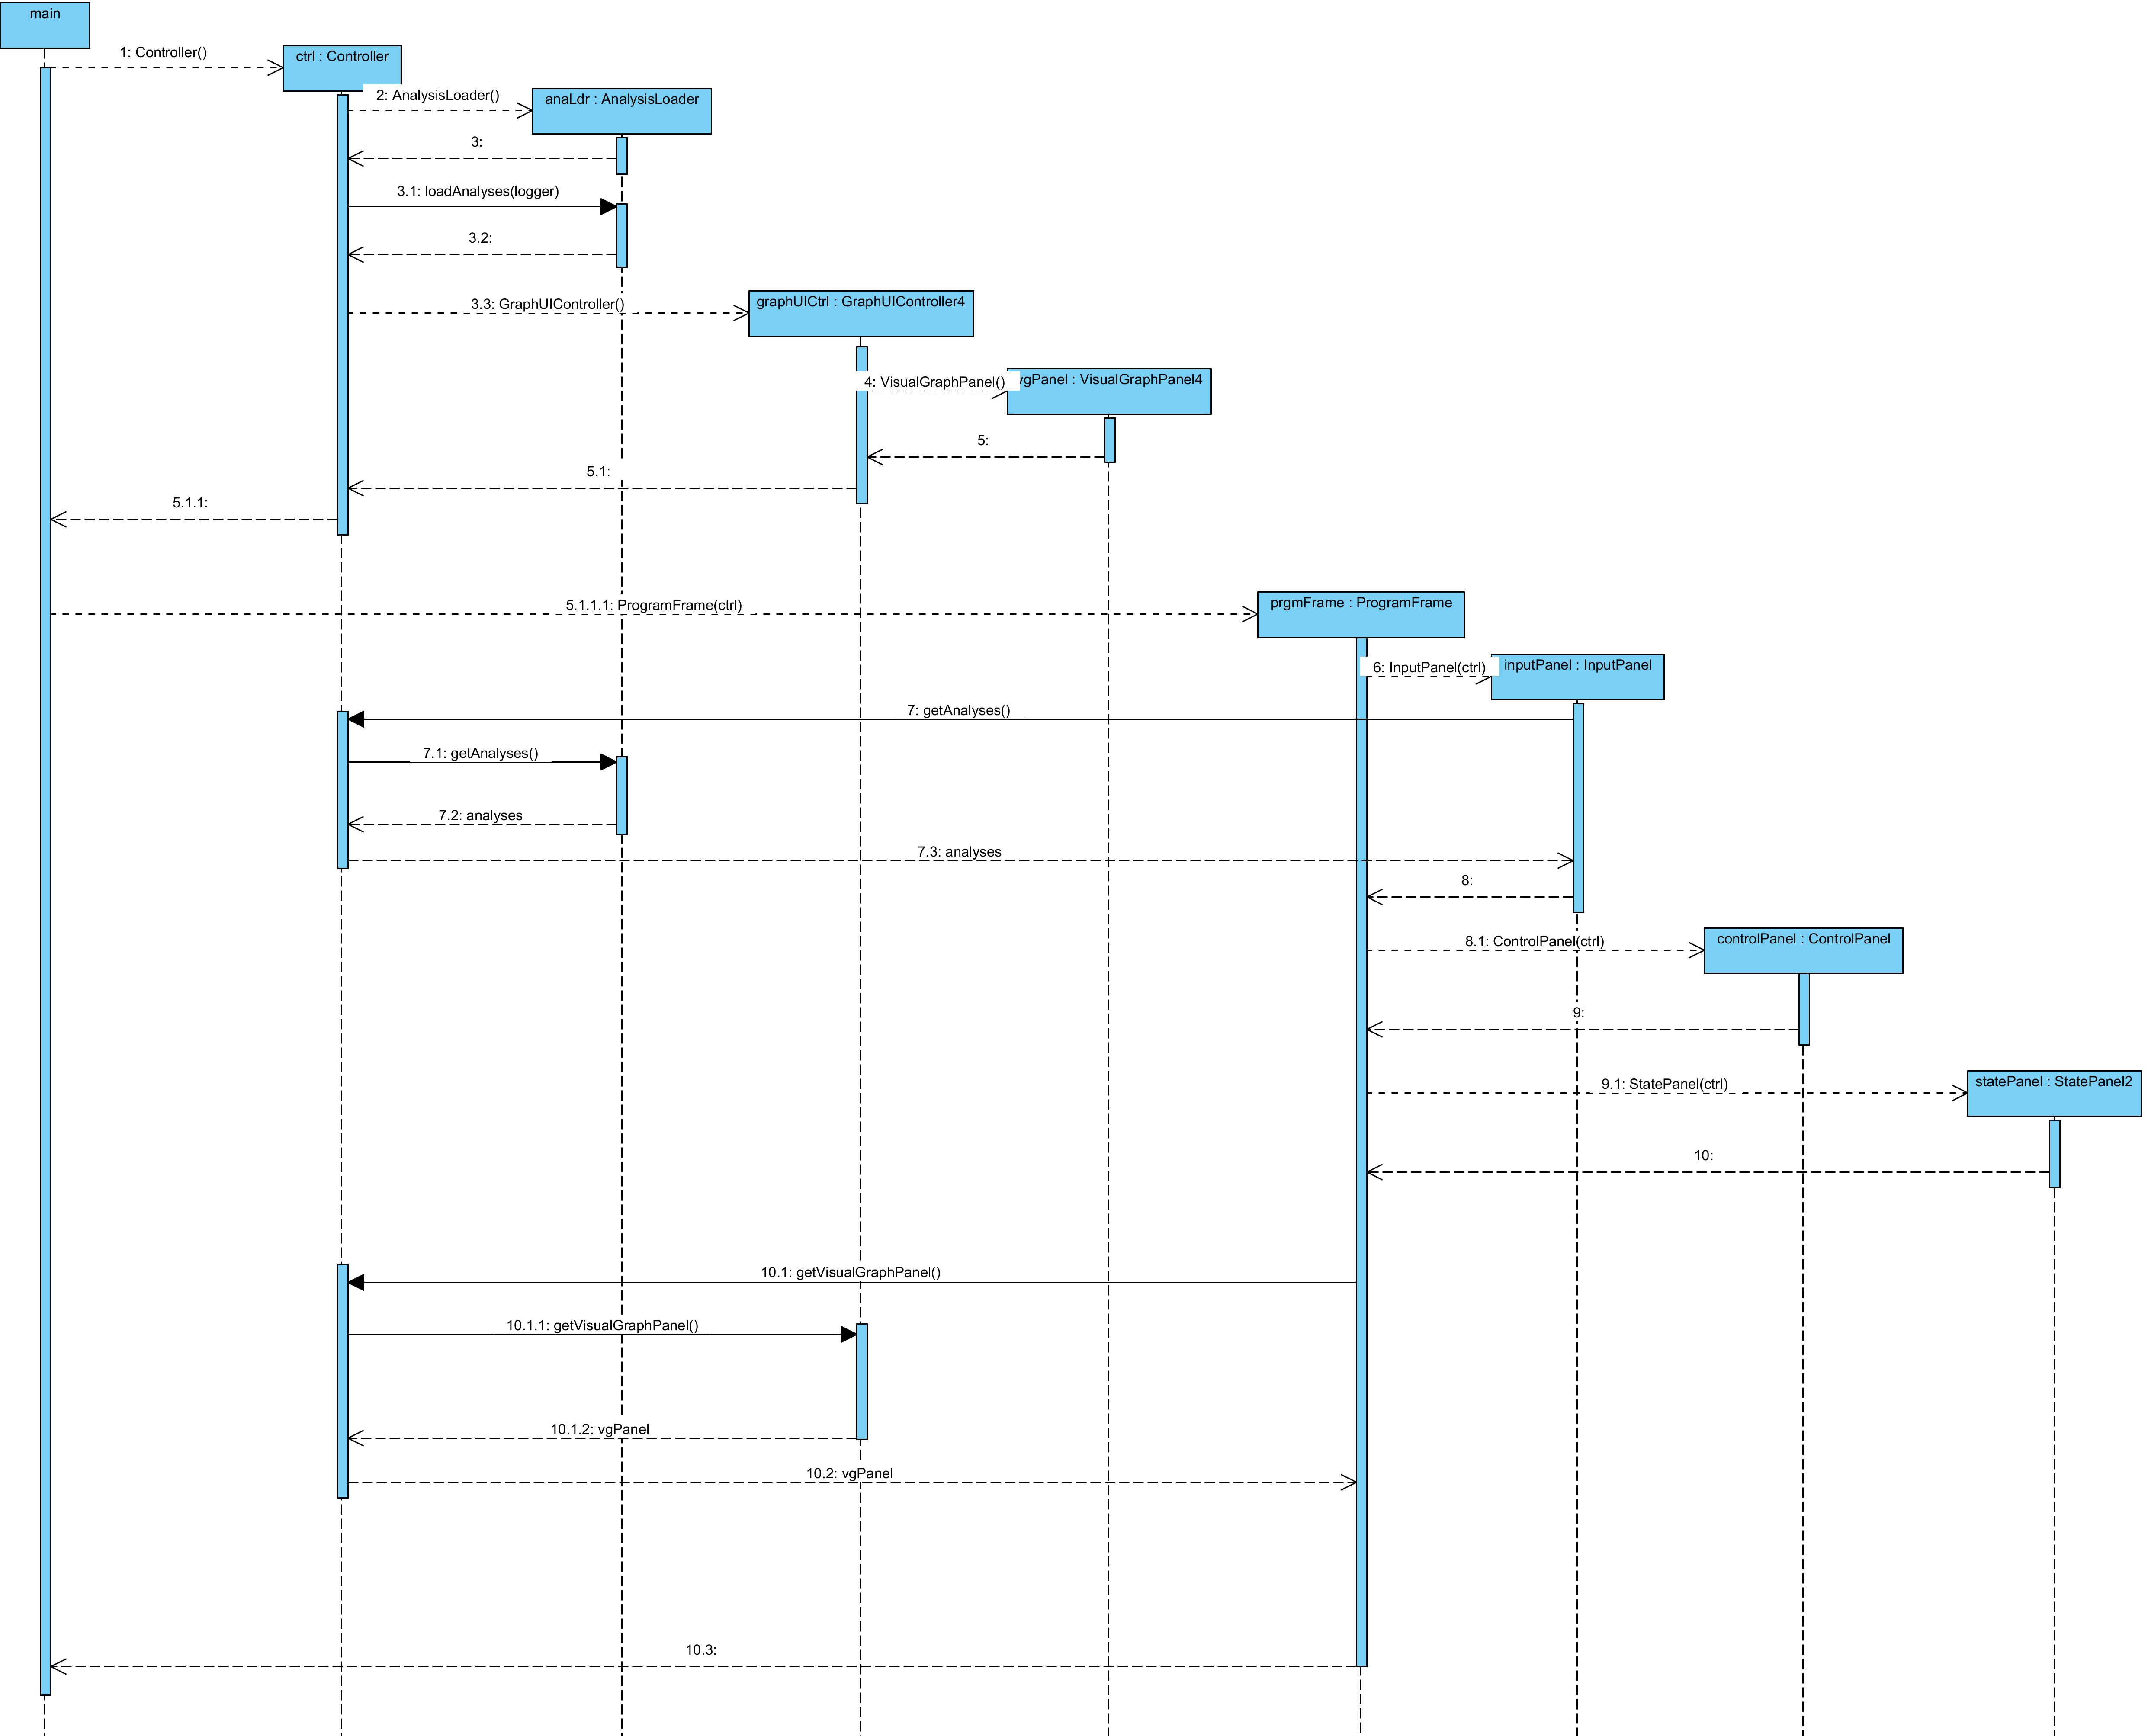
\includegraphics[width=1\textwidth]{Sequenzdiagramme/ProgramStart}
  \caption{Starten des Programms}
  \label{fig:start}
\end{figure}
\FloatBarrier
\clearpage


\section{Konstruktor der DFAExecution}
\clearpage


\section{Erstellen eines neuen Graphen}
\begin{figure}[!htp]
  \centering
    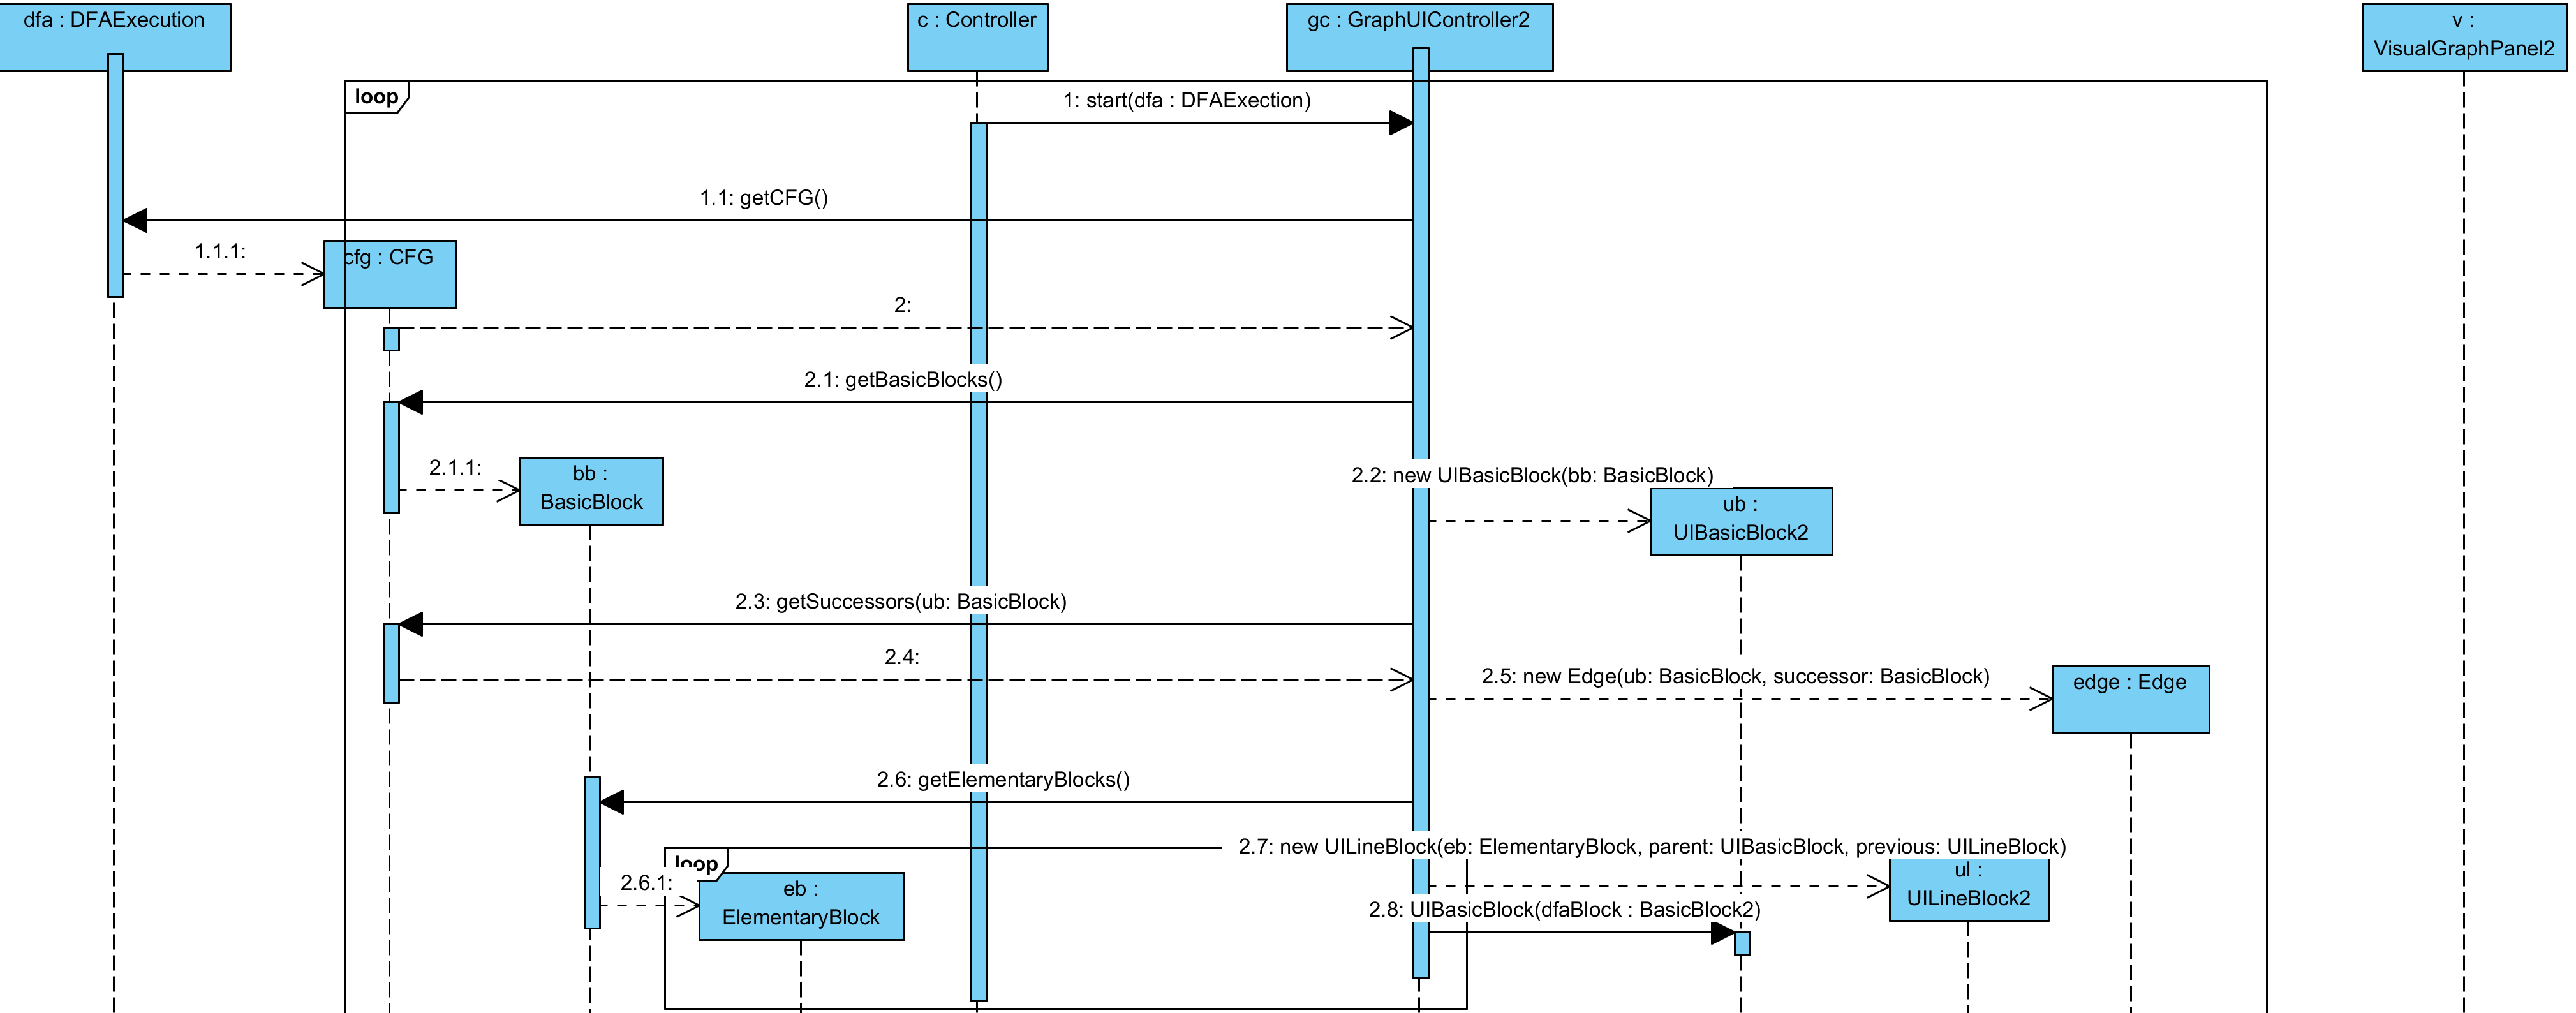
\includegraphics[width=1\textwidth]{Sequenzdiagramme/CreateNewGraph}
  \caption{Konstruktor der DFAExecution}
  \label{fig:constructor}
\end{figure}
\newpage
\clearpage

\section{Starten der Analyse}
\begin{figure} [!htp]
  \centering
    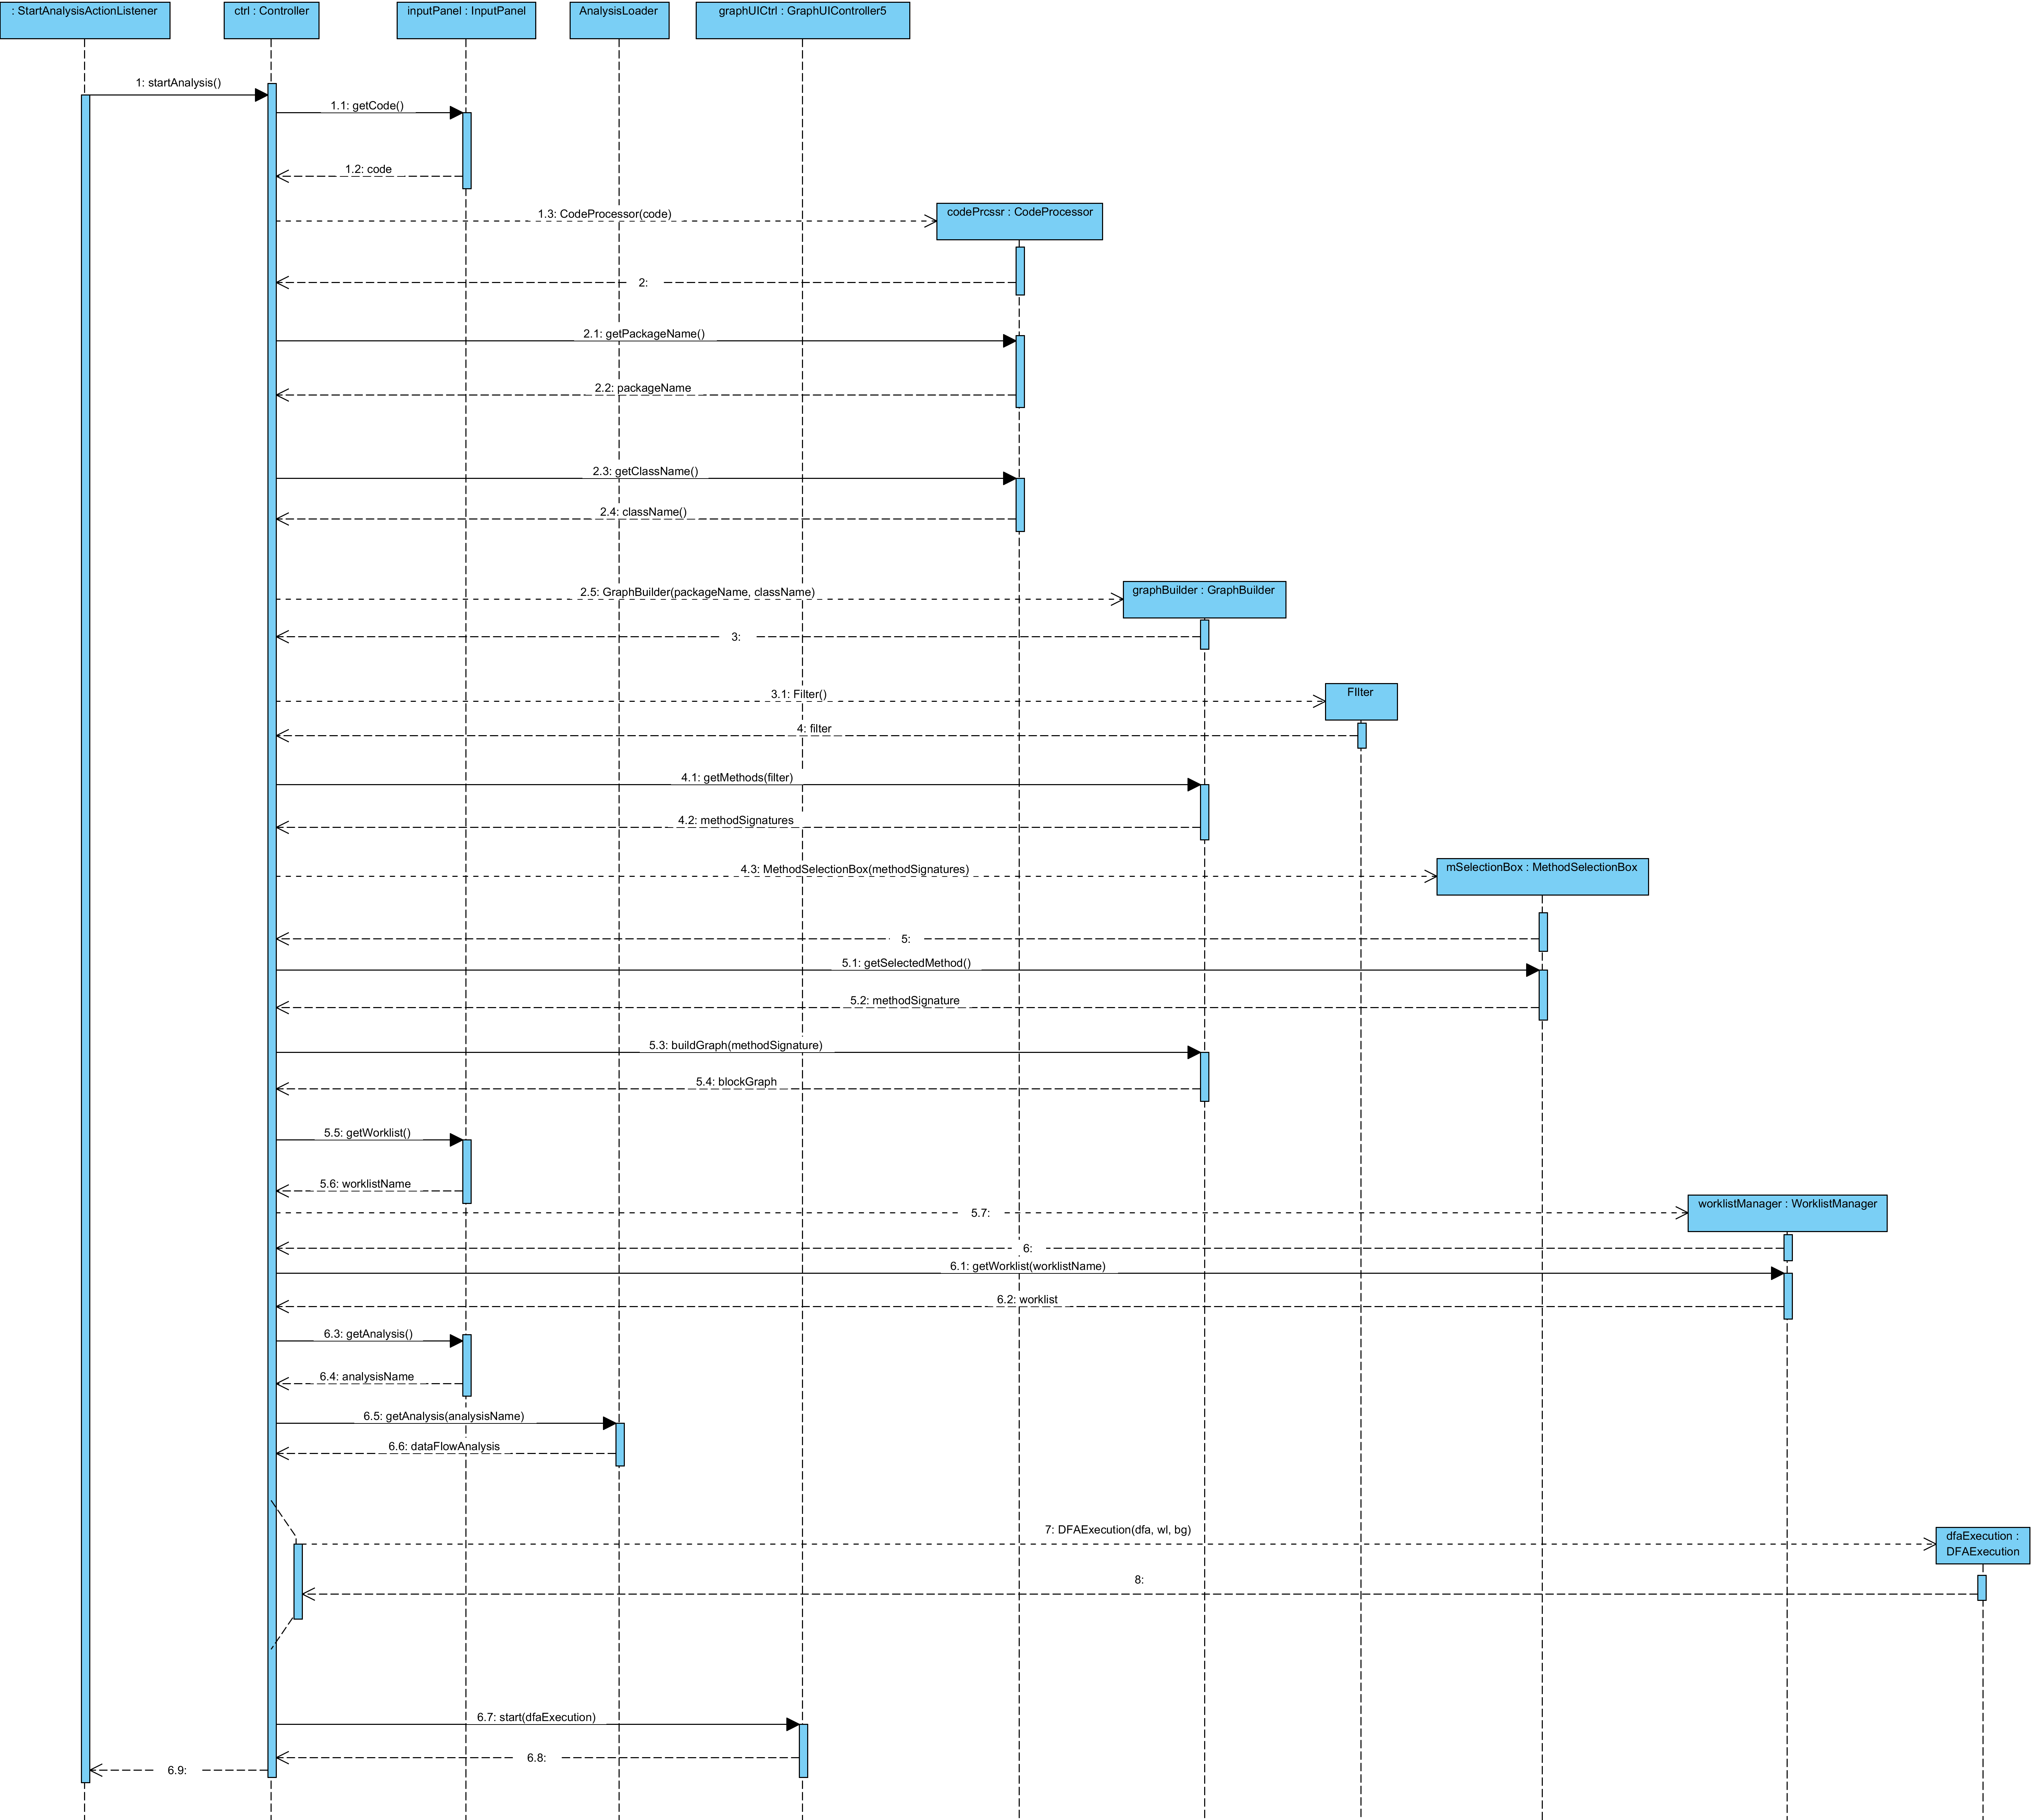
\includegraphics[width=1\textwidth]{Sequenzdiagramme/AnalysisStart}
  \caption{Starten der Analyse}
  \label{fig:anaStart}
\end{figure}
\FloatBarrier
\clearpage

\section{Stoppen der Analyse}
\begin{figure}[!htp]
  \centering
    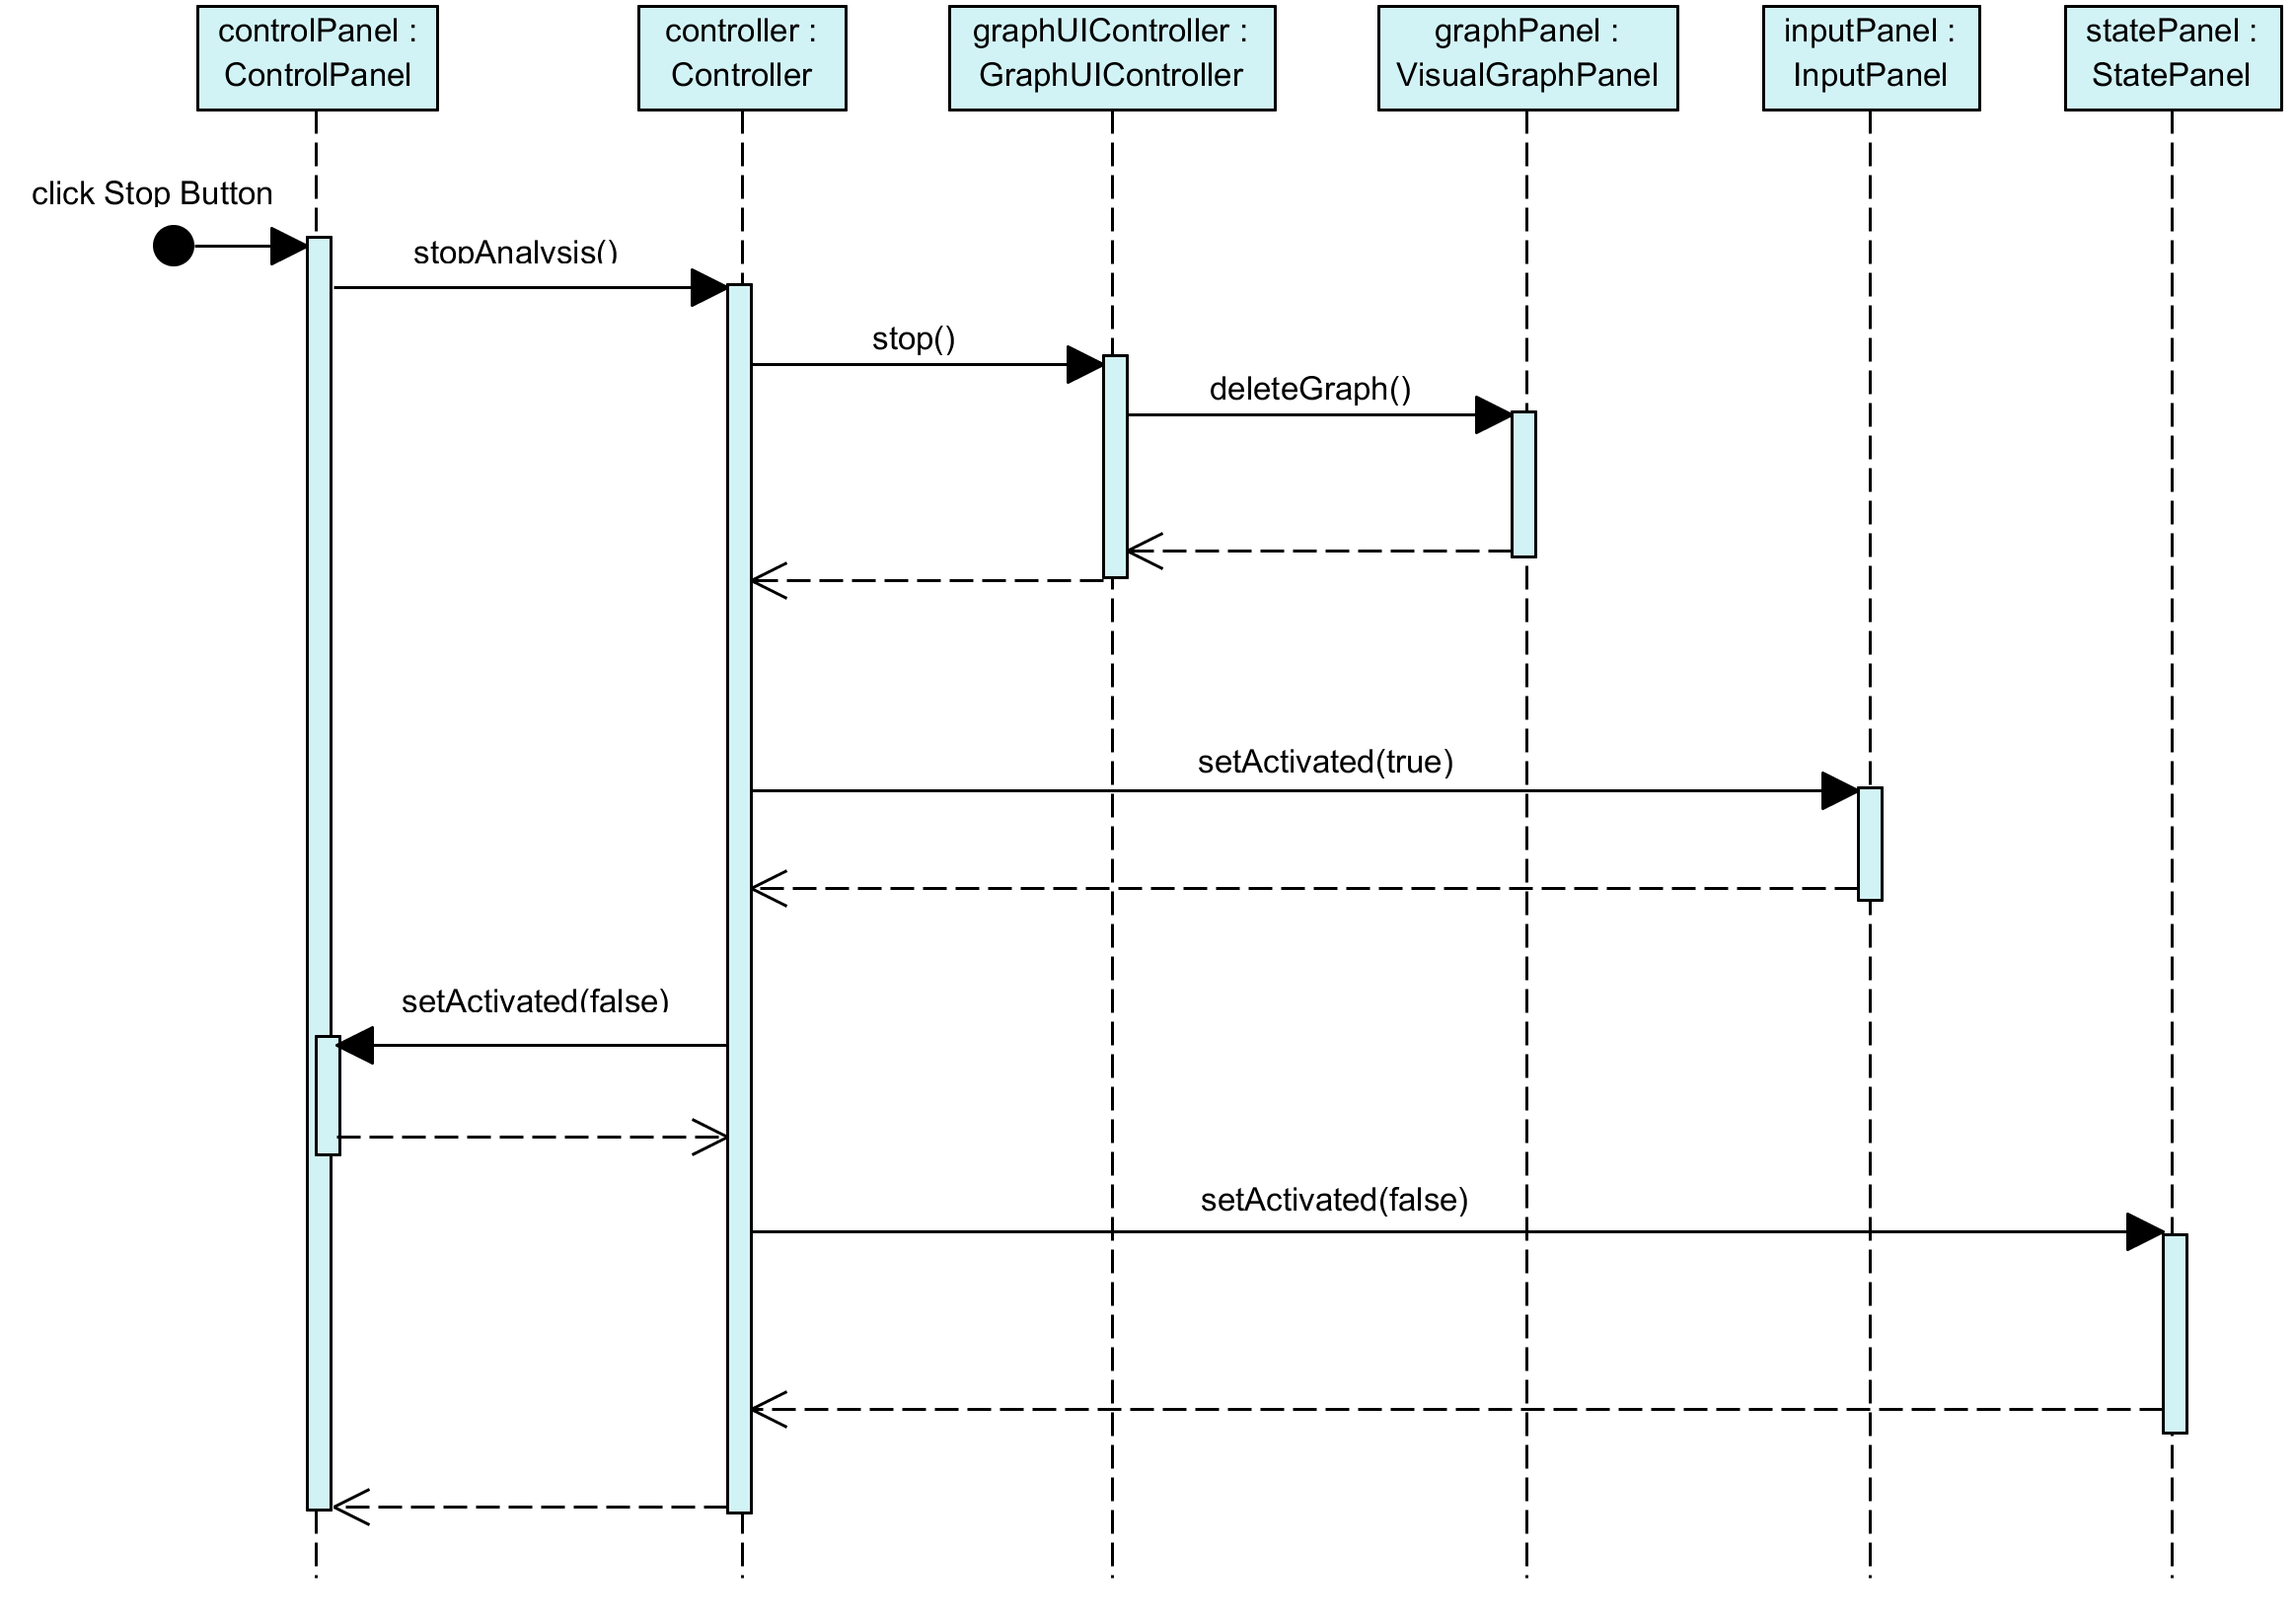
\includegraphics[width=1\textwidth]{Sequenzdiagramme/AnalysisStop}
  \caption{Stoppen der Analyse}
  \label{fig:anaStop}
\end{figure}
\clearpage

\section{Den folgenden Block analysieren}
\begin{figure}[!htp]
  \centering
    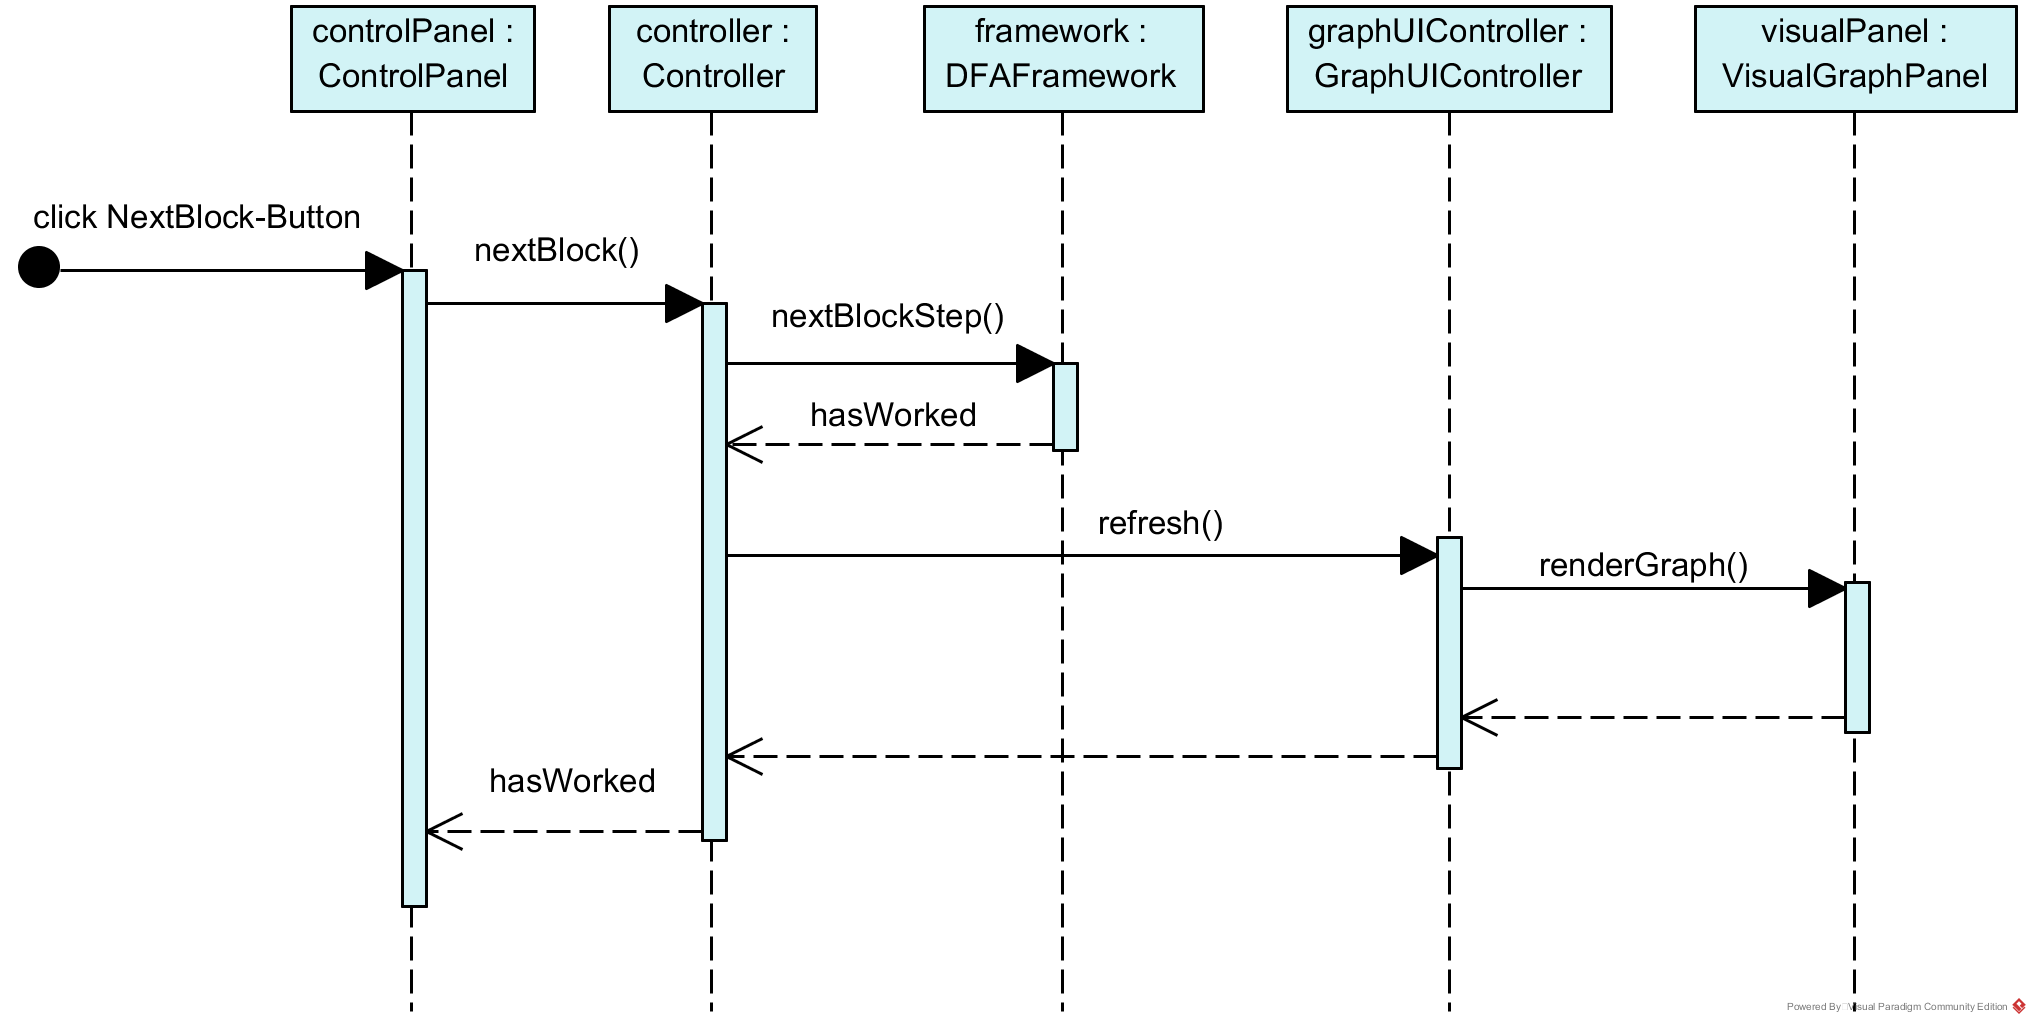
\includegraphics[width=1\textwidth]{Sequenzdiagramme/NextBlock}
  \caption{Den folgenden Block analysieren}
  \label{fig:nextblock}
\end{figure}
\FloatBarrier
\clearpage

\section{Breakpoint setzen}
\begin{figure}[!htp]
  \centering
    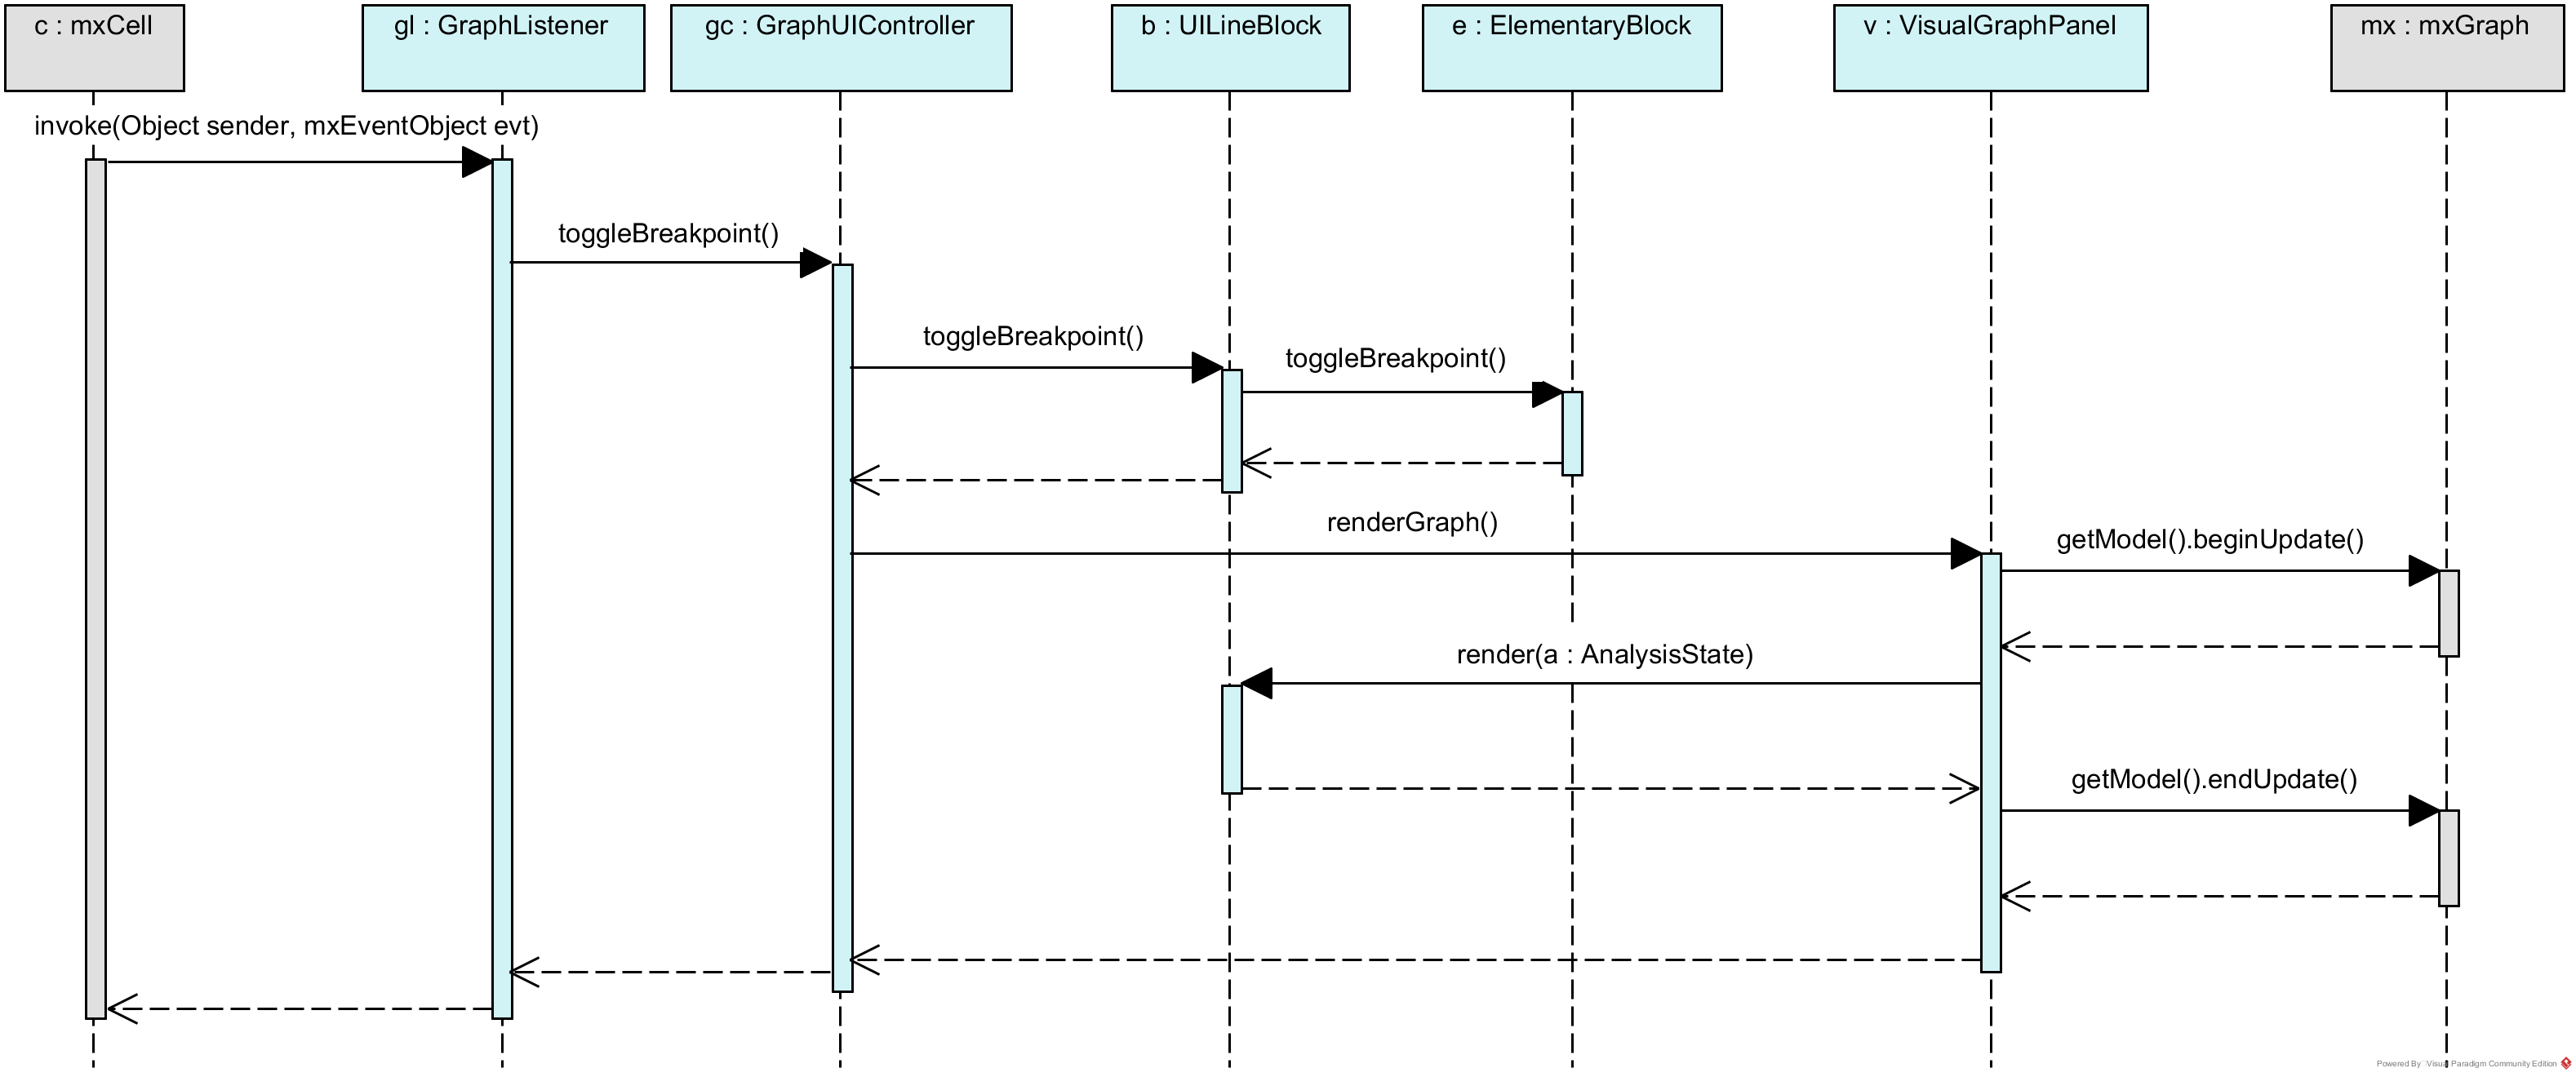
\includegraphics[width=1\textwidth]{Sequenzdiagramme/SetBreakpoint}
  \caption{Breakpoint setzen}
  \label{fig:breakpoint}
\end{figure}
\clearpage
\FloatBarrier